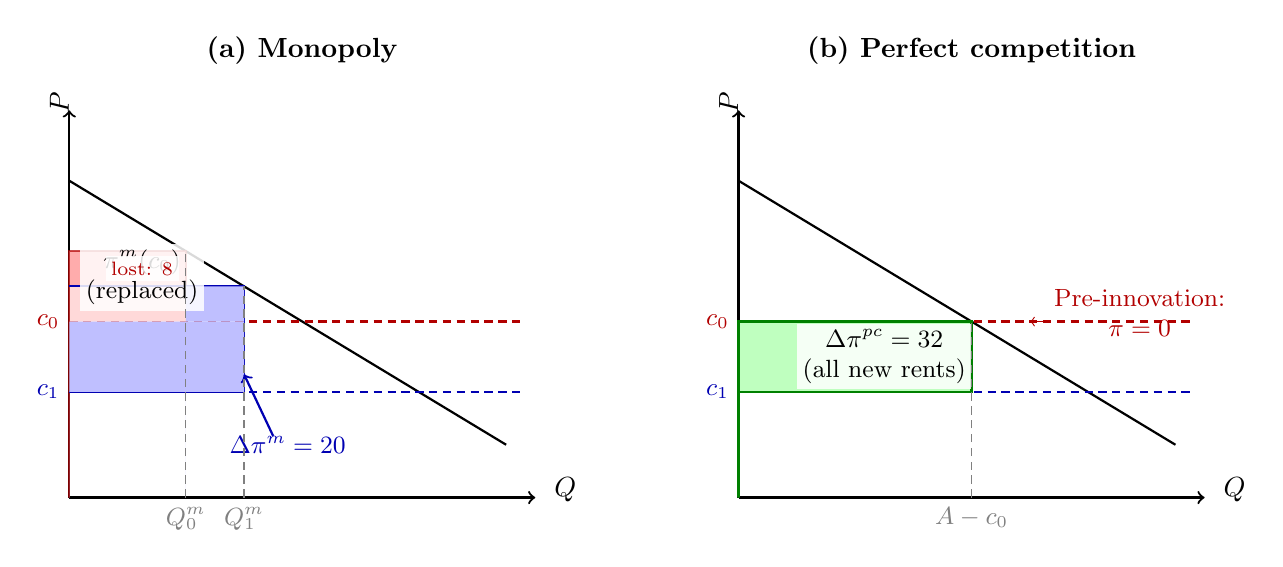
\begin{tikzpicture}
% Two-panel figure: Monopoly (left) vs Perfect Competition (right)
% Shows why competitive innovator gains MORE than monopolist

% === Panel A: Monopoly ===
\begin{scope}[xshift=0cm]
\begin{axis}[
  name=panelA,
  width=7.5cm, height=6.5cm,
  xmin=0, xmax=16,
  ymin=0, ymax=22,
  axis lines=left,
  axis line style={thick, ->},
  ticks=none,
  clip=false,
  xlabel={$Q$},
  ylabel={$P$},
  xlabel style={at={(axis description cs:1.02,0.02)}, anchor=west},
  ylabel style={at={(axis description cs:0.02,1.02)}, anchor=south},
  title={\textbf{(a) Monopoly}},
  title style={at={(0.5,1.05)}, anchor=south},
]

% Parameters: A=18, c0=10, c1=6
\pgfmathsetmacro{\A}{18}
\pgfmathsetmacro{\cO}{10}
\pgfmathsetmacro{\cI}{6}
\pgfmathsetmacro{\QmO}{(\A-\cO)/2}  % 4
\pgfmathsetmacro{\PmO}{(\A+\cO)/2}  % 14
\pgfmathsetmacro{\QmI}{(\A-\cI)/2}  % 6
\pgfmathsetmacro{\PmI}{(\A+\cI)/2}  % 12

% Demand curve
\addplot[thick, domain=0:15, samples=2] {\A - x};

% Cost lines
\addplot[thick, densely dashed, red!70!black, domain=0:15.5, samples=2] {\cO};
\addplot[thick, densely dashed, blue!70!black, domain=0:15.5, samples=2] {\cI};
\node[anchor=east, red!70!black, font=\small] at (axis cs:0,\cO) {$c_0$};
\node[anchor=east, blue!70!black, font=\small] at (axis cs:0,\cI) {$c_1$};

% Pre-innovation profit (light red): rectangle c0 to P^m(c0), width Q^m(c0)
\addplot[fill=red!15, draw=none, forget plot]
  coordinates {(0,\cO) (\QmO,\cO) (\QmO,\PmO) (0,\PmO)} \closedcycle;

% Lost profit strip (top-left of old rectangle, darker red with pattern)
\addplot[fill=red!40, draw=red!70!black, thick, forget plot, opacity=0.7]
  coordinates {(0,\PmI) (\QmO,\PmI) (\QmO,\PmO) (0,\PmO)} \closedcycle;

% Post-innovation profit (blue outline): rectangle c1 to P^m(c1), width Q^m(c1)
\addplot[draw=blue!70!black, thick, fill=none, forget plot]
  coordinates {(0,\cI) (\QmI,\cI) (\QmI,\PmI) (0,\PmI)};

% Net gain = blue area minus red area
% Shade only the INCREMENTAL gain (blue minus red overlap)
% Top strip: P^m(c0) to P^m(c1) is GONE (P^m(c1) < P^m(c0) since c1<c0)
% Here: P^m(c1) = 12, P^m(c0) = 14
% The incremental gain is: new rectangle - old rectangle

% Shade the gain region: parts of blue not in red
% Bottom strip: c1 to c0, width Q^m(c1)
\addplot[fill=blue!25, draw=none, forget plot]
  coordinates {(0,\cI) (\QmI,\cI) (\QmI,\cO) (0,\cO)} \closedcycle;

% Right strip: Q^m(c0) to Q^m(c1), c0 to P^m(c1)
\addplot[fill=blue!25, draw=none, forget plot]
  coordinates {(\QmO,\cO) (\QmI,\cO) (\QmI,\PmI) (\QmO,\PmI)} \closedcycle;

% Labels (drawn AFTER fills to ensure visibility)
% Pre-innovation profit label
\node[font=\small, align=center, fill=white, fill opacity=0.85, text opacity=1, inner sep=2pt] at (axis cs:2.5,12.5) {$\pi^m(c_0)$\\(replaced)};
% Lost profit label
\node[font=\scriptsize, red!70!black, fill=white, fill opacity=0.85, text opacity=1, inner sep=2pt] at (axis cs:2.5,13) {lost: 8};
% Delta pi^m label with arrow to blue region
\node[font=\small, align=center, blue!70!black] at (axis cs:7.5,3)
  {$\Delta\pi^m = 20$};
\draw[->, blue!70!black, thick] (axis cs:7,3.5) -- (axis cs:6,7);

% Dashed verticals with x-axis labels
\addplot[densely dashed, thin, gray] coordinates {(\QmO,0) (\QmO,\PmO)};
\node[anchor=north, gray, font=\small] at (axis cs:\QmO,0) {$Q^m_0$};

\addplot[densely dashed, thin, gray] coordinates {(\QmI,0) (\QmI,\PmI)};
\node[anchor=north, gray, font=\small] at (axis cs:\QmI,0) {$Q^m_1$};

\end{axis}
\end{scope}

% === Panel B: Perfect Competition ===
\begin{scope}[xshift=8.5cm]
\begin{axis}[
  name=panelB,
  width=7.5cm, height=6.5cm,
  xmin=0, xmax=16,
  ymin=0, ymax=22,
  axis lines=left,
  axis line style={thick, ->},
  ticks=none,
  clip=false,
  xlabel={$Q$},
  ylabel={$P$},
  xlabel style={at={(axis description cs:1.02,0.02)}, anchor=west},
  ylabel style={at={(axis description cs:0.02,1.02)}, anchor=south},
  title={\textbf{(b) Perfect competition}},
  title style={at={(0.5,1.05)}, anchor=south},
]

% Parameters
\pgfmathsetmacro{\A}{18}
\pgfmathsetmacro{\cO}{10}
\pgfmathsetmacro{\cI}{6}
\pgfmathsetmacro{\Qpc}{\A - \cO}  % 8 (non-drastic: limit price at c0)

% Demand curve
\addplot[thick, domain=0:15, samples=2] {\A - x};

% Cost lines
\addplot[thick, densely dashed, red!70!black, domain=0:15.5, samples=2] {\cO};
\addplot[thick, densely dashed, blue!70!black, domain=0:15.5, samples=2] {\cI};
\node[anchor=east, red!70!black, font=\small] at (axis cs:0,\cO) {$c_0$};
\node[anchor=east, blue!70!black, font=\small] at (axis cs:0,\cI) {$c_1$};

% Pre-innovation: P = c0, profit = 0 (nothing to shade)
\node[font=\small, red!70!black, align=center, anchor=west] at (axis cs:10.5,10.5)
  {Pre-innovation:\\$\pi = 0$};
\draw[->, red!70!black] (axis cs:10.5,10) -- (axis cs:10,10);

% Post-innovation profit (non-drastic): rectangle c1 to c0, width A-c0
\addplot[fill=green!25, draw=green!50!black, thick, forget plot]
  coordinates {(0,\cI) (\Qpc,\cI) (\Qpc,\cO) (0,\cO)} \closedcycle;

% Label the profit
\node[font=\small, align=center, fill=white, fill opacity=0.85, text opacity=1, inner sep=2pt] at (axis cs:5,8)
  {$\Delta\pi^{pc} = 32$\\(all new rents)};

% Dashed vertical at Q = A - c0
\addplot[densely dashed, thin, gray] coordinates {(\Qpc,0) (\Qpc,\cO)};
\node[anchor=north, gray, font=\small] at (axis cs:\Qpc,0) {$A-c_0$};

\end{axis}
\end{scope}

\end{tikzpicture}
